\begin{center}
  \Large
  \textbf{BIOGRAFI PENULIS}
\end{center}

\addcontentsline{toc}{chapter}{BIOGRAFI PENULIS}

\vspace{2ex}

\begin{wrapfigure}{L}{0.3\textwidth}
  \centering
  \vspace{-3ex}
  % Ubah file gambar berikut dengan file foto dari mahasiswa
  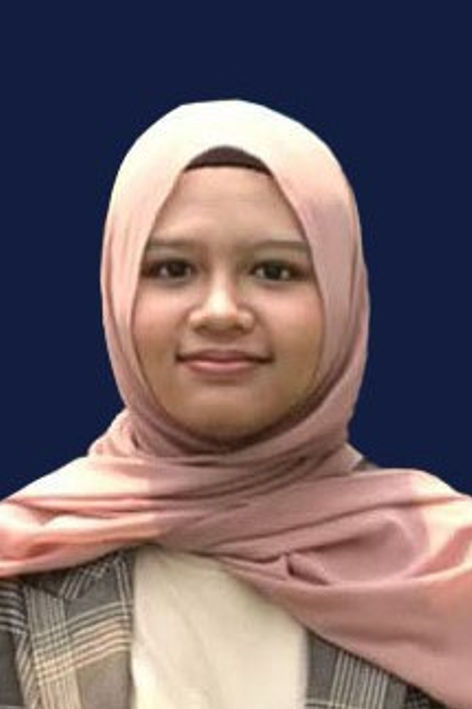
\includegraphics[width=0.3\textwidth]{gambar/Batrisyia Zahrani Ananto 5024201065 4 x 6.jpg}
  \vspace{-4ex}
\end{wrapfigure}

% Ubah kalimat berikut dengan biografi dari mahasiswa
Batrisyia Zahrani Ananto, lahir pada 01 April 2002 di Jakarta. Penulis merupakan anak pertama dari dua bersaudara. Setelah lulus dari SMA Negeri 8 Jakarta, penulis kemudian melanjutkan pendidikan ke jenjang strata satu di Departemen Teknik Komputer, Fakultas Teknologi Elektro dan Informatika Cerdas, Institut Teknologi Sepuluh Nopember mulai tahun 2020.
